
\documentclass[final,11pt,a4paper,twocolumn,oneside]{article}

\usepackage[utf8]{inputenc}

\usepackage{amsmath}
\usepackage{amsfonts}
\usepackage{amssymb}
\usepackage{graphicx}
\usepackage{array}
\usepackage{booktabs}
\usepackage{float}
\usepackage{newclude}
\usepackage{bm}
\usepackage{pdfpages}

\usepackage[binary-units=true]{siunitx}
\usepackage[colorlinks,allcolors=blue]{hyperref}
\usepackage[font={small,it}]{caption}
\usepackage[font={small,it}]{subcaption}
\usepackage[hmargin={0.7in,0.6in},vmargin={0.9in,1.1in}]{geometry}

\edef\restoreparindent{\parindent=\the\parindent\relax}
\usepackage{parskip}
\restoreparindent

\usepackage[natbib=true,backend=biber,sorting=none]{biblatex}
\bibliography{references}

\usepackage{mathtools}
\DeclarePairedDelimiter{\abs}{\lvert}{\rvert}

\interfootnotelinepenalty=10000
\raggedbottom
% \raggedright

% \setcounter{topnumber}{8}
% \setcounter{bottomnumber}{8}
% \setcounter{totalnumber}{8}

% \sisetup{range-units=single}
% \sisetup{range-phrase=\kern 0.08333em--}

\hyphenation{quad-ru-poles quad-ru-pole}

\title{\bfseries Simulating the Measurement of the\\
Electron Beam Emittance at AWAKE}
\author{Patrick~Chin}

\begin{document}

\twocolumn[
	\begin{@twocolumnfalse}
		\vspace*{15em}
		\maketitle
		\thispagestyle{empty}
		\vspace*{5em}
		\begin{center}
			Department of Physics \& Astronomy, \\
			University College London \\
			% Gower Street, London, WC1E 6BT \\
			\vspace*{6em}
			Supervised by Prof.~M.~Wing \\ \& Dr.~S.~Jolly \\
		\end{center}
	\end{@twocolumnfalse}
]

% \clearpage
% 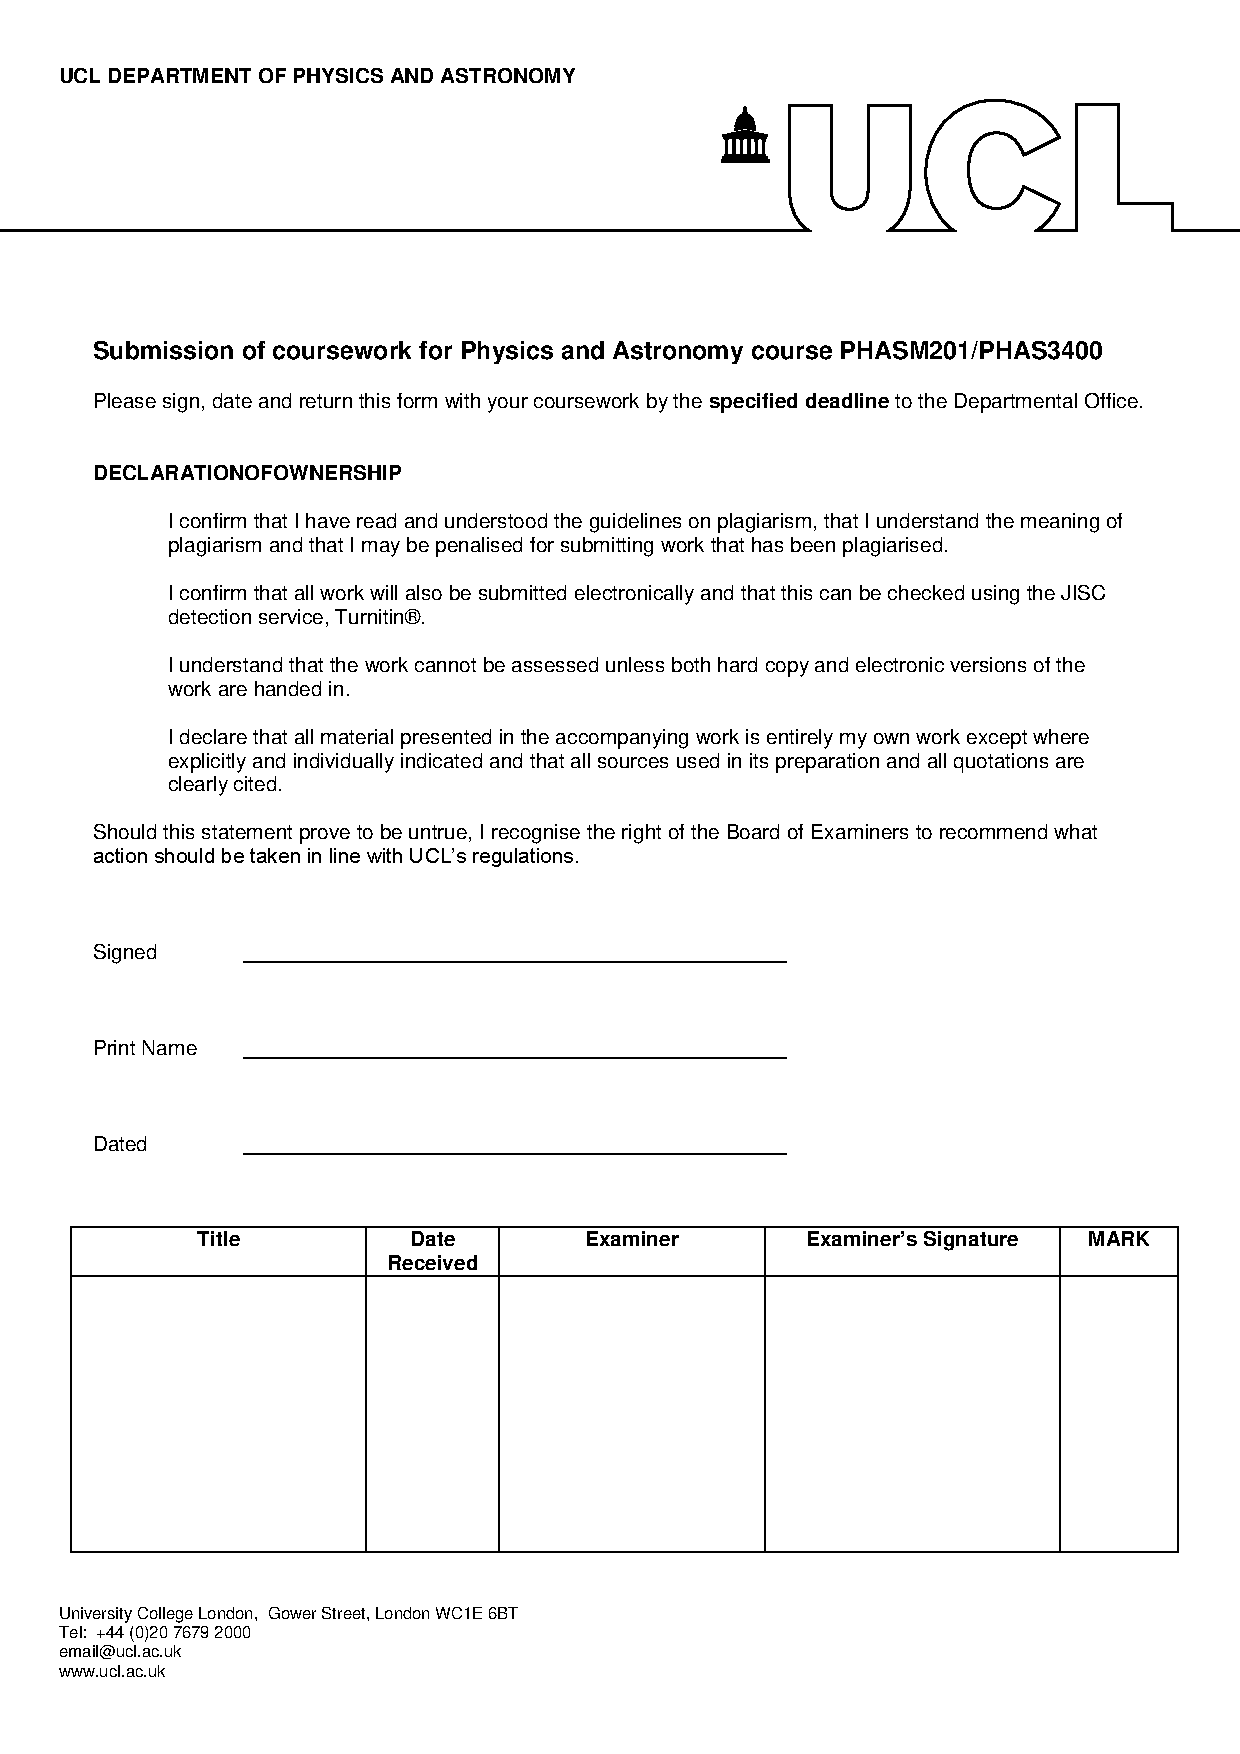
\includepdf{declaration.pdf}

\twocolumn[
	\begin{@twocolumnfalse}
	\thispagestyle{empty}
	\vspace*{15em}

		\begin{center}
			\section*{Abstract}
		\end{center}
		In preparation for experiments at AWAKE in CERN, simulations of the beam
		and measuring of the beam's parameters were carried out.  This was done
		in order to investigate how the measurement of the emittance of the beam
		behaves under changes to experimental parameters.  The energy spread of
		the beam was investigated and a minimum percentage energy spread of
		\SI{4}{\percent} was found to be the cutoff point at which measurements
		become reliable. Emittance values were investigated and emittances above
		\SI{e-5}{\meter\radian} were found to be measured inaccurately.
		Background photon values up to \num{e4} times the expected background
		were simulated, showing accurate measurements up to a factor of
		\num{\sim4e2}, above which the measured emittance deviated significantly
		from the true value. Improvements and limitations of the simulation due
		to assumptions made are also discussed.

	\end{@twocolumnfalse}
]

\clearpage
\twocolumn[
	\begin{@twocolumnfalse}
		\thispagestyle{empty}
		\hypersetup{allcolors=black}
		\tableofcontents
	\end{@twocolumnfalse}
]
\clearpage

% \pagenumbering{arabic}
\include*{introduction}
\include*{awake}
\include*{spectrometer}
\include*{theory}
\include*{simulation}
\include*{results}
\include*{conclusion}
% 
% % \appendix
% \begin{appendices}
% \part{Code}
% \end{appendices}


% \clearpage
\printbibliography

\end{document}

